\documentclass[a4paper]{article}
\usepackage{graphicx} % Required for inserting images
\usepackage{enumerate}% http://ctan.org/pkg/enumerate
\usepackage[superscript,biblabel]{cite}

\title{Thermoacoustic heat pumps}
\author{Thomas Meylaers}
\date{April 2023}

\newcommand{\newpara}
    {
      \bigbreak{}
      \noindent
    }

\begin{document}

\maketitle

\newpage

\begin{abstract}

\end{abstract}

\newpage

\tableofcontents

\newpage


\section{Introduction} % read paper on room temperature applications
Thermoacoustic heat pumps (TAHP) are a new and upcoming technology. This technology offers an environment-friendly and efficient solution for heating applications.
\newpara{}
In contrast to traditional heating and cooling applications which rely on the vapor compression cycles, TAHP uses the energy stored in sound waves to transfer heat between temperature reservoirs. These mechanisms have a relatively simple design compared to their more-traditional counterparts. TAHP also use more environment-friendly working media such as helium and hydrogen.
Working on these principles, this technology has the potential to offer significant advantages over traditional heating and cooling methods, including reduced energy consumption, lower maintenance costs, and reduced environmental impact.\cite{powerofsound}
\newpara{}
This paper will first discuss the physics behind these systems in section X. Section X discusses the applications of TAHP with the difference between standing wave and traveling wave principles in mind. Subsequently, section X discusses the challenges and possible shortcomings of TAHP.\@ This paper will conclude in section X with final remarks.

\section{Working principles}
\subsection{Standing Waves\cite{powerofsound,enginesandrefrigerators,tijaniLoudSpeaker}}
In a standing wave, gas parcels alternatively compress and expand. This process happens adiabatically. These compressions and expansions change the temperature and pressure of these gas parcels. When the pressure reaches maximum so does the temperature and vice versa.
\newpara{}
These temperature variations are relatively small. For sounds at 120 \(dB\), the temperature oscillates up and down by only about 0.02 degrees Celcius. Most air conditioners and refrigerators need to pump heat over a range of 20 degrees or more. So the temperature changes within the gas are too small to be useful.
\newpara{}
To handle larger temperature ranges TAHP put the gas in contact with a solid. A solid has a much higher heat capacity per unit volume than gas and can absorb a considerable amount more heat without changing temperature very much. The solid absorbs heat when a gas parcel compresses and moves to the left. The solid will release heat to a gas parcel when it drops in temperature due to expansion and moves to the right. A temperature gradient is created along the solid. The temperature gradient due to this gas parcel is very small, but when multiple of these gas parcels are all undergoing this process, they work as a sort of bucket brigade bringing heat from one side to the other. % FIGURE
This cycle for a gas parcel plotted in a \(p-V\) diagram shows that there is work absorbed by the gas and is typical for a heat pump.  % FIGURE
This process can be reversed where a temperature gradient along the solid is provided by an outside source which is then converted into acoustic power. Such a device is called a \emph{thermoacoustic heat engine (TAHE)} or \emph{primer mover}.
\newpara{}
The solid used in TAHP should have good thermal contact when the parcel is stationary but poor thermal contact when the parcel is moving. The solid should not conduct heat from one end to the other and thus have a low conductivity. The quest of finding this material is a large part of making TAHP commercially viable, but plastic is often sufficient for experimental applications.
\newpara{}
TAHP use a stack of plates of the solid previously discussed called the \emph{stack}. These plates are mounted parallel to each other. Detailed analysis shows that the optimal distance between these plates is about four times the \emph{thermal penetration depth} \(\delta_\kappa = \sqrt{\kappa/\pi f \rho c_p}\). % DISCUSS THIS FURTHER
\newpara{}
The most rudimentary form of a TAHP consists of a resonator, gas, stack, acoustic transducer, and hot and cold heat exchangers. The acoustic transducer applies acoustic power \(W\) to the gas in the resonator such that a standing wave of the first harmonic is formed in the resonator. A stack is located at about a fourth of the resonator length from the transducer. A hot heat exchanger is mounted on the left at the side of the stack which is closest to the node where temperature and pressure will be at their maximum. A cold heat exchanger is then mounted on the right side closest to the anti-node.
\newpara{}
The gasses used in TAHP are typically noble gasses such as helium, neon, argon, or a mixture of these gases. These gasses are used because they have low molecular weights and are highly compressible, which makes them ideal for use in thermoacoustic refrigerators. Additionally, they have low thermal conductivity, which helps to minimize heat transfer between the hot and cold sides of the device.
\newpara{}
The bucket brigade of gas parcels pumps heat from the cold end of the stack to the hot end and creates a temperature gradient. In the case of a \emph{thermoacoustic refrigerator}, the cold exchanger is connected to a room to be cooled at \(T_c\), and the hot exchanger is connected to a heat sink at \(T_h\). This is reversed when the desired effect is the heating of a room. This technology is, however, the most promising in the former case.

\subsubsection{Efficiency and losses}
The efficiency for heat pumps, known as the \emph{coefficient of performance (COP)}, is limited by the second law of thermodynamics and is defined by the Carnot efficiency \(T_c/(T_h-T_c)\). The losses preventing this device from reaching Carnot efficiency are as follows:
\begin{description}
  \item[Inherent losses] Inherent losses are due to the irreversibility of the heat transfer between the stack and a gas parcel. Because the heat transfer happens across a non-zero temperature difference \(\delta T\), the entropy of the universe increases. This irreversibility is inherent to this device because of the imperfect thermal contact. % ADD FORMULA
  \item[Viscous losses] Viscous losses occur because the gas must overcome viscous shear forces in the stack. The \emph{viscous penetration depth} \(\delta_\mu=\sqrt{\mu / \pi f \rho} \) is comparable to the \emph{thermal penetration depth} \(\delta_\kappa\). Because the plates are spaced about four times this depth apart, the gasses undergo a significant amount of viscous shear.
  \item[Conduction losses] This loss occurs by the simple conduction of the hot end of the stack to the cold end of the stack.
  \item[Auxiliary losses] The losses discussed also happen in other parts of the device. Viscous and inherent losses also occur in other parts of the resonator, not necessarily in the stack, which also contributes to the losses. Conduction losses also occur through the casing of the resonator.
  \item[Transduction Losses] The acoustic transducer generating power for the system is also imperfect. In the case of an electrical system, i.e. a loudspeaker, the main losses will be Joule heating in the copper wires of the loudspeaker.
\end{description}

These losses combined cause simple standing-wave TAHP to be inefficient. A stereo configuration developed by Garrett\cite{powerofsound} and his colleagues for the US Navy to cool radar electronics only achieved 17\% of the Carnot efficiency. The refrigerator itself, however, achieved 26\% of the maximum which is only half of what conventional cooling systems of similar shape can achieve. % FIGURE
\newpara{}
Standing wave TAHP should, however, not be immediately discarded. The efficiency of these devices can still be improved. Furthermore, almost no moving parts are required. In the case where a loudspeaker is used only a simple seal like a metal bellow would suffice and there would be no need for lubrication. There is also the possibility of coupling the TAHP with a thermoacoustic heat engine which means that there would be no moving parts at all. In this configuration, waste heat from e.g. an industrial installation would power a thermoacoustic heat engine producing acoustic power which would then be fed to a TAHP to cool down or heat a space for example.
\newpara{}
The efficiency of standing wave systems is imposed by the way that heat is transferred from the stack to the gas which is similar to the Brayton cycle. Researchers have found a way to use a different thermodynamic cycle, the Stirling cycle, to improve the efficiency of thermoacoustic devices.\cite{ceperleyStirling}
The COP of traditional vapor compression refrigerators generally ranges between 2 and 6 whilst the COP of a traveling wave TAHP is between 1 and 1.2.\cite{Herman2006,tijaniOptimalStack}
% Should add more information like figures, graphs, and variations

\subsection{Traveling Waves\cite{spoelstraHighTemperature,BackHauseDetailedStudy,powerofsound,weiTravellingwave}}
In contrast to the inherently irreversible thermodynamic cycle which standing wave TAHP use, the reversed Stirling cycle is inherently reversible. By finding a TAHP which uses this reverse Stirling cycle it is possible to surpass the efficiency of standing wave TAHP.\@

\subsubsection{Stirling cycle}
The Stirling cycle for a Stirling engine with a regenerator consists of four different steps:
\begin{enumerate}[i]
  \item 1→2 Isothermal heat addition (expansion)
  \item 2→3 Isochoric heat removal (constant volume)
  \item 3→4 Isothermal heat removal (compression)
  \item 4→1 Isochoric heat addition (constant volume)
\end{enumerate}
This cycle in a \(p-V\) diagram is shown in Figure X. The connection between traveling acoustic waves and a Stirling engine becomes clear when the temperature gas and velocity are plotted alongside each other for the acoustic wave and the gas in the regenerator of the Stirling engine. The changes in pressure and velocity of the gas in the regenerator resemble those of a traveling acoustic wave.
\newpara{}
Ceperley\cite{ceperleyStirling} showed that a TAHE could be created by creating a temperature gradient across a regenerator and sending a traveling wave through it. Ceperley was not successful in building a device that could do this efficiently, but through years of research and experimentation by his peers, TAHE using traveling waves became the most efficient and promising form of TAHE.\@ As with standing wave TAHE, when the cycle is reversed a TAHP is created.

\subsubsection{Traveling wave TAHP\cite{TARTIBU2019102}}
One of the main differences between a traveling wave and a standing wave TAHP is the regenerator. The regenerator is a porous solid with a high heat capacity. These pores are smaller than the thermal penetration depth and thus much smaller than the gaps in a stack. These smaller pores, however, ensure better thermal contact and makes it possible for the device to be reversible in theory.
\newpara{}
The losses in the regenerator are proportional to the square of the oscillating velocity of the gas. This is analogous to the power dissipated in an electrical resistor which is proportional to the square of the current. Electrical engineers solved this similar problem for transmission lines by lowering the current and increasing the voltage. Garrett and Backhaus\cite{powerofsound} reasoned that the way electrical engineers solved this problem could also apply to the acoustically analogous case. This means that the velocity of the gas should be minimized and the oscillatory pressure should be maximized to increase efficiency. A traveling wave TAHP should thus have a wave that has the oscillatory pressure and velocity in phase whilst also minimizing the oscillatory velocity in the regenerator. Standing waves have a high pressure-to-displacement ratio, a traveling wave TAHP should thus incorporate the best of both worlds to maximize efficiency.
\newpara{}
A widely adopted design for traveling wave TAHP combines a standing wave resonator and a torus-like device containing the regenerator (See figure X). The torus is comprised of a hot heat exchanger (HHX), a regenerator (REG), a cold heat exchanger (CHX), a thermal buffer tube (TBT), an ambient heat exchanger (AHX), and a feedback inertance. The standing wave in the resonator moving along the open end of the torus acts like air blowing over the mouth of a bottle. The springiness of the gas in the inertance tube allows a wave of high pressure and low displacement (standing wave property) with the velocity and pressure in phase (traveling wave) to develop. The combination of these properties makes this specific configuration one of the most efficient methods of thermoacoustic refrigeration. The acoustic network formed by these elements forces a traveling wave to travel anti-clockwise in the torus and make the gas perform a reverse Stirling cycle in the regenerator and thus pumping heat away from the CHX.\@ The TBT and AHX are there to prevent heat from leaking.\cite{TijaniAHighPerformanceThermoacousticEngine}.
\newpara{}
One major problem with this design is that it does not inhibit Gedeon streaming i.e.\ air circulating from one end of the loop to the other and thus short-circuiting the CHX and HHX.\@ This phenomenon drastically impacts efficiency and should be avoided. A flexible membrane installed just above the HHX would inhibit the flow of gas whilst still transmitting the acoustic power but can be difficult to develop in such a way that it lasts a long time. Another way is to use a jet pump. A jet pump creates a backpressure in the loop to inhibit the streaming by using asymmetric openings that allow flow in one direction.

\subsubsection{Efficiency}
Various designs have been tested numerically or experimentally since Ceperly first wrote his paper in 1979. The most promising are the looped-based designs as discussed above but efficiencies are still poor and insufficient for commercial viability. There are also different aims of these devices. Some traveling wave TAHP have been designed to liquefy hydrogen where cooling power is important while some designs focus more on room temperature applications where efficiency and power density are important\cite{WangRoomTemperature}.
\newpara{}
Tijani et al.\cite{spoelstraHighTemperature} built a traveling wave TAHP by building on the design discussed above. They coupled the TAHP with a TAE using the same principle but with a reversed cycle. This makes this device thermally driven. They managed to get to 40\% of Carnot's performance working between a range of 80 degrees and 10 degrees Celcius and pumping 200 W. This was an encouraging result for further study in this domain.
\newpara{}
Luo et al.\ built a refrigerator using the design discussed above\cite{LuoRefrigerator}. They also did this by coupling a traveling wave TAHP with a TAE in the same system but in a different way than the previous example. This device only reached a COP of 0.216 but managed to pump 469 W.
\newpara{}
More recently, Wang et al.\ estimated numerically that a refrigerator could be built with a cooling power of 6.35 kW and a COP of 3. This was built on the principle of putting multiple regenerators in series and thus creating a multistage refrigerator. Real-world experimentation is required however to validate these results.
\newpara{}
An in-depth study on the efficiency of traveling wave TAHP by Ueda et al.\ showed that three parameters mainly affect the efficiency of the regenerator: the regenerator's installation position, length, and flow-channel radius\cite{uedaOptimization}. They concluded that by optimizing these three parameters a COP of above 60\% of the Carnot COP could be achieved. Tartibu investigated the effect of different geometries and thus configurations of traveling wave TAHP and tabulated different findings of different researchers\cite{TARTIBU2019102}. His study shows that whilst traveling wave TAHP are not sufficiently efficient yet, they show great promise and have much higher potential than their standing wave counterparts.

\section{Applications}
This section will discuss real-world applications of TAHP.\@ There are not a lot of real-world applications outside of academia because of the infancy of this technology.
\subsection{Space applications}
Thermoacoustic applications are a good fit for space missions because of their reliability and energy density. In this section, I list two important applications.
\subsubsection{Space shuttle get-away-special (GAS)\cite{AdeffSpace,powerofsound}}
Two standing-wave TAHP were designed, tested, and certified by NASA for its launch of the GAS space shuttle in 1992. One component was devised to cool the urine and blood samples of astronauts the other component was designed to cool electronic components. The TAHP had the stereo configuration as discussed above and used a mixture of helium and xenon as the working gas. The devices achieved 16\% of Cartnot's COP which was impressive considering the novelty of the technology. Due to an abrupt stop of funding the project was never realized. Due to the promising technology, it was later picked up by the US Navy to cool radar electronics.
\subsubsection{JWT cryocooler\cite{Petach2014MidII,Moore_2017,ross2022conceptual}}
The James-Webb telescope (JWT) is a space telescope launched by NASA on 25 December 2021. The purpose of JWT was to conduct infrared astrology. Due to redshift, the light coming from very old and distant celestial bodies have a wavelength in the infrared range. The temperature of the mid-infrared camera (MIRI) aboard the JWT has to be as close to 0 kelvin as possible to minimize the infrared radiation of the telescope itself and thus minimize the noise.
\newpara{}
The heat shield of the JWT only manages to keep the temperature of the sensor at about 37 kelvin but the sensor has an operating temperature of 6.2 kelvin. NASA chose a thermoacoustic cooler because reliability, high cooling power, and energy density were key. The cryocooler is a standing wave TAHP operating on helium with three stacks. A tube of helium is connected to the cold heat exchangers of the TAHP and is cooled down to about 17 kelvin which is still not enough which is still not sufficient. At the end of the tube, there is a small hole that drops the pressure of the helium. Because of this Joule-Thompson effect, the helium cools down to 6.2 kelvin to finally cool the MIRI.\@ So far, this cooler has worked successfully and is expected to for the coming 18 years.

\subsection{Domestic applications}
Almost 80\% of domestic heating in Europe is still being done with fossil fuels according to the EU\cite{EU}. There are two startups in Europe seeking to improve these numbers by making heat pumps a more accessible and environment-friendly option.
\subsubsection{Blue Heart\cite{blueheart}}
Blue Heart is a Dutch spinoff of the Organisation for Applied Scientific Research (TNO). A Blue Heart device would replace the cold circuit of a heat pump. The high energy density of TAHP reduces the space needed for heat pump installations. They developed a traveling wave TAHP with helium as the working fluid. The acoustic power is generated by two pistons opposite to each other moving at the same frequency. The vibrations get canceled making the TAHP more silent than their conventional compression-based counterparts. Blue Heart claims that its device works efficiently with every temperature input and output and has a larger operation envelope than compression-based heat pumps. They also claim to be compatible with every type of heat source and to be suitable for new and existing houses.
\newpara{}
A Blue Heart device would operate with source temperatures between -20 degrees to 50 degrees Celsius and with sink temperatures between 7 degrees and 80 degrees Celsius. It would also have a capacity of 6 kW. The company plans to make the device commercially available in 2024.
\subsubsection{Equium\cite{equium}}
Equium is a French startup that offers to replace the heat pump entirely in contrast to Blue Heart. The company has not revealed the inner workings of their device but it is expected to also be a traveling wave TAHP working with helium. The company promises an impressive maintenance-free lifetime of 30 years. These devices are also planned to be commercially available in 2024
\subsection{Automotive applications}
Current refrigeration and cooling systems in automotive applications, based on compression, draw a lot of power from the engine and degrades the overall efficiency of the vehicle. Furthermore, the refrigerant often leaks from the system and is made of ozone-depleting material. An environment-friendly and efficient alternative to cooling systems in vehicles is thus crucial.
\newpara{}
Zoontjens et al.\ did a feasibility study on TAHP in automotive applications\cite{zoontjens2005feasibility}. They specifically studied the possibility of a thermally driven TAHP driven by recovered waste heat from waste exhaust gasses. They also compared this alternative to other prominent alternatives such as active magnetic resonator systems, solid adsorption cooling systems, vapor absorption refrigeration systems, etc.  What makes TAHP appealing, in this case, is the possibility to be driven thermally because combustion engines have low thermal efficiencies and thus release a significant amount of heat to the environment. A diagram of the system they devised is shown in Figure~\ref{automotiveDiagram} (ATAR stands for automotive thermoacoustic refrigeration).
\begin{figure}[h]
  \centering
  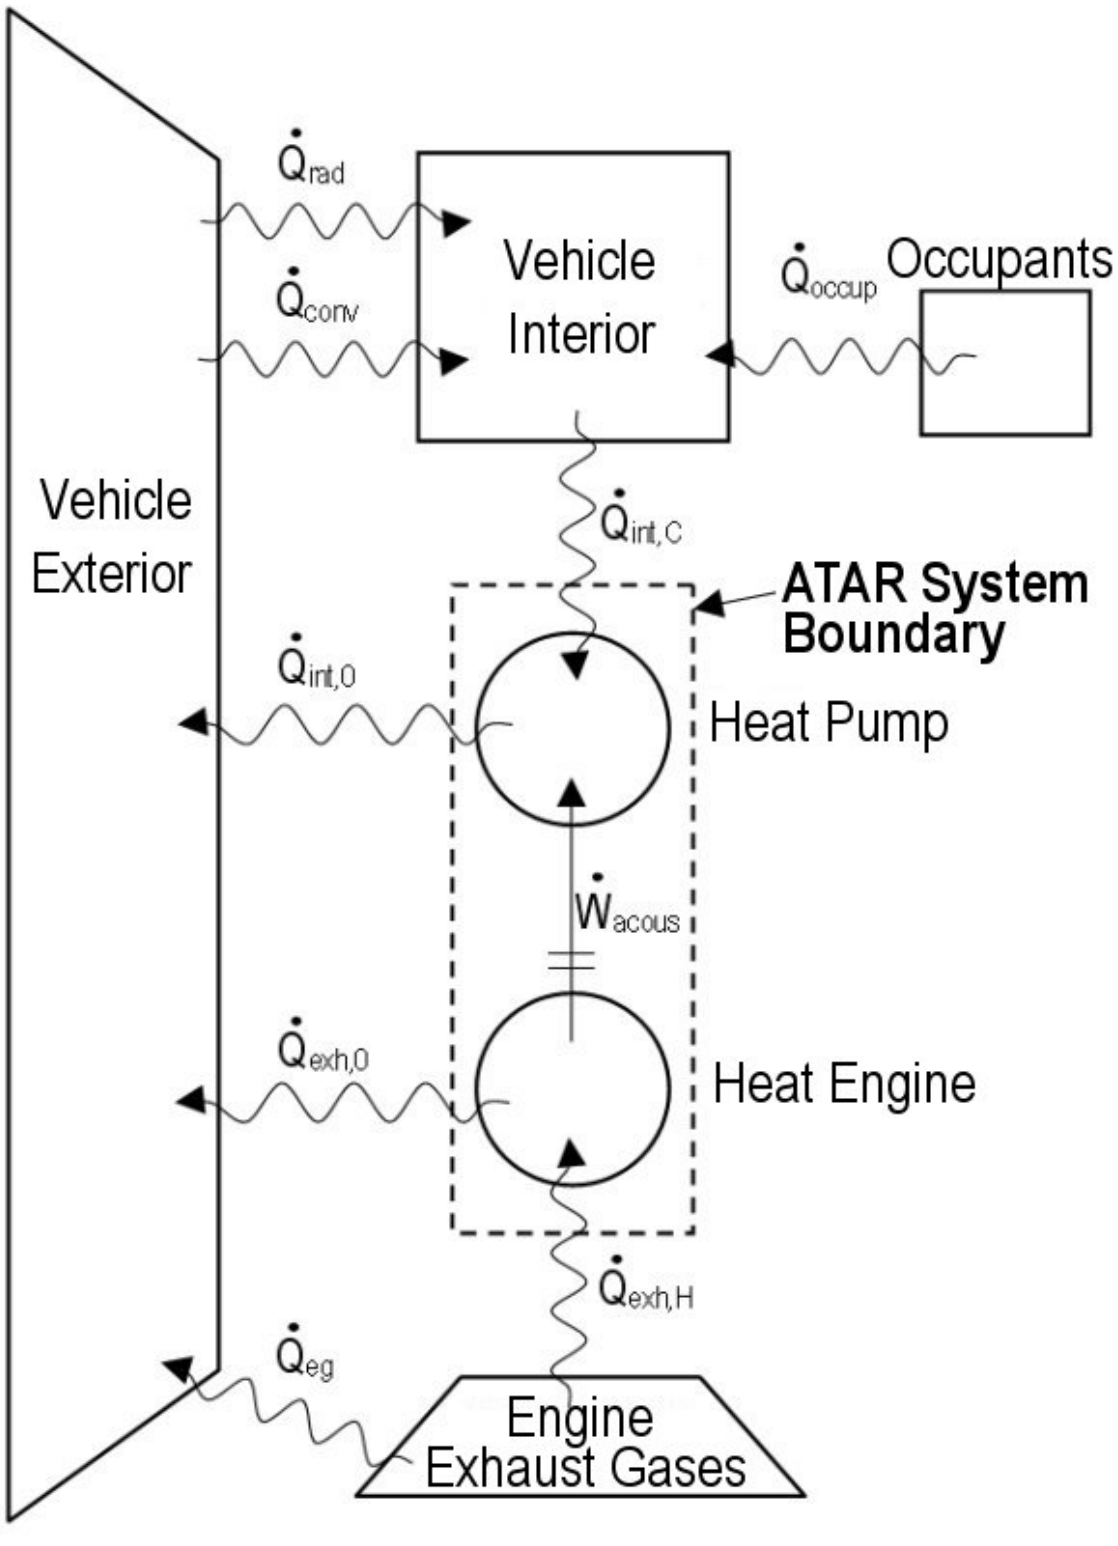
\includegraphics[width=0.5\textwidth]{images/automotive.png}
  \caption{Diagram of automotive thermoacoustic refrigerator\cite{zoontjens2005feasibility}}\label{automotiveDiagram}
\end{figure}
The implementation chosen for this study was a standard quarter-wavelength standing wave TAHP as discussed above. The two major concerns are cooling power and available heating power. The cost of developing a production-ready system of this kind is a big challenge to overcome. Especially with the ever-decreasing demand for combustion engine vehicles. The researchers found that these systems would be feasible but that further optimization and research will be necessary.
\section{Future challenges and limitations}

\section{Conclusion}
While efficiencies are not yet at the same levels as conventional cooling/heating applications, one should keep in mind that TAHP offers other important advantages. For example, they use inert gases which make them environment friendly. They are also very flexible in driver methods. They can be powered thermally and mechanically. They also have nearly no moving parts which makes them very suitable for environments where reliability is key.
\newpage
\bibliography{uni}
\bibliographystyle{unsrt}
\end{document}
